%-------------------------------------------------------------------------------
\section{Design}
%-------------------------------------------------------------------------------
\sys's design centers around the key observation that user data may expose identifying information
both directly from its contents, and indirectly through its structural correlations to other
application data. \sys must therefore pinpoint exactly which data and correlations may be
identity-sensitive, and allow developers to specify exactly what the post-unsubscription state of
the data should be.

In order to capture exactly which data contents, and which data correlations may be
identity-sensitive, \sys models an application's data as a graph of \emph{entity} nodes and edges.
Each entity type corresponds to an application datatable, such as a stories, users, or votes table.
Entities are linked in the entity graph by foreign key relationships: table columns that act as
foreign keys to other tables create child-parent relationships between entities.  \sys also includes
abstract entities in the graph, where the keys may be non-referential identifiers that refer to
abstract, non-table entities (e.g.,\ a \texttt{thread\_id} column in the comments table).  Edges in
the graph---foreign or abstract key relationships---represent correlations between the nodes of the
graph, namely individual entities.

Unsubscription policies center around the abstraction of \emph{ghost entities}. A ghost entity is
more than an anonymized version of a real entity: a real entity may be replaced by multiple ghost
entities, breaking up correlations associated with the real entity; and ghost entities can be partially
randomized, partially custom generated, and partially clones of the real entities, achieving
fine-grained data retention and anonymization. Pre- and post-unsubscription state differ by the
presence of ghost entities nodes and edges to ghost entities, which have taken the place of real
entities and edges to these entities.

While \sys operates on a specific instance of the application entity graph, the developer reasons
only about the \emph{types} of individual entities and the \emph{types} of entity edges that may be
instantiated in the graph. This allows unsubscription policies to be specified statically using only
the application schema, while \sys ensures that any instance of the application entity graph
satisfies the state specified in the policy.

\subsection{Ghosting Entity Attributes}
Developers must first define how ghost entities are generated from a real entity.
\sys assumes entities have three kinds of attributes: a unique identifier attribute; 
value (non-referencing) attributes (such as a timestamp or username), and 
edge (referential foreign key) attributes that identify correlations to parent entities. 
Value attributes may directly expose identifying information from its
contents, and edge attributes represent potentially sensitive structural correlations. 

For every entity type, developers specify \emph{value ghosting policies} that apply at per-column
granularity to non-referencing attributes. Value ghosting policies take as input a current entity's
attribute value, and return a ghosted version. Developers can specify whether the ghosted
replacement should be random, a default value, or generated from the original value via a custom
function provided by the developer. 

For each edge attribute of the entity type, the developer specifies an 
\emph{edge ghosting policy} that specifies how and when the edge can be decorrelated.
%Using ghost generation policies, \sys creates ghost entities to replace unsubscribed entities. 

Ghost entities always have unique values for their identifier attribute.

%During unsubscription, \sys traverses the current instance of the application entity graph with the
%top-level unsubscribing user node as the root in order to find all possible graph edges and nodes
%that may be sensitive. \sys then applies the applies the appropriate decorrelation policy to all
%sensitive edges depending on the edge type, generating ghost nodes with ghosted attributes to
%replace real nodes as specified.
%
%After ghosts are generated from the template entity, \sys returns a copy of the template entity to
%the unsubscribing user, which if returned upon resubscription, allows \sys to restore the original
%value. If the user does not wish to store this data, resubscription retains the ghosted value in
%%place of the original.
%Resubscription requires the user to return the original
%data to restore the original value.

\subsection{Edge Ghosting Policies}
Edge ghosting policies are specified on a particular edge type (a parent entity type and a child
entity type). In database terms, edge ghosting policies are specified on referencing
(foreign key) columns, namely the edge attributes of entity types.

Developers can choose between options to either replace correlations with correlations 
to ghost parents; retain correlations but ghost the attributes of the parent nodes; remove
correlations entirely; or add false correlations to introduce noise. 
The following sections explain each in more detail.

\paragraph{Policy 1: Decorrelate.}
Application developers specify that edges of this type should be decorrelated. \sys identifies all groups of
children entities (of the edge's child type) that have foreign keys to the same parent (of the
edge's parent type). For each child in the same group, \sys creates a ghost parent entity using
the shared parent as a template entity, and
rewrites the child's key attribute value to be the new ghost parent's identifier. 

To generate ghost parent entities' non-referencing attributes, developers can choose between the options, which apply at per-column
granularity:
\begin{itemize}
    \item \textbf{Clone-All:} All ghost parents share the same value for this column attribute as the
        template parent.
    \item \textbf{Generate-All:} \sys uses the ghost attribute policy for this column to
        generate the attribute value for all ghost parents.
    \item \textbf{Clone-One:} One ghost parent shares the same value for the column attribute as the
        template; \sys uses the ghost attribute policy for this column to
        generate the attribute value for all other ghost parents.
\end{itemize}

All generated ghost entities initially clone the values of referencing---foreign key---attributes of the template parent entity. 
\sys then looks up the appropriate decorrelation policy for that parent-to-grandparent edge type, and applies it to all the generated
ghost parents. For example, if the parent entity has a decorrelatable edge to a grandparent entity,
then all ghost parent entities will be re-linked to ghost grandparent entities.
%If the column represents a foreign key into another table, then either the referenced table must 
%have a ghost generation policy, or the foreign key is set to an existing entity or
%placeholder ghost.
%(the foreign key is set to point to ``deleted story''). 
%It is up to the developer to ensure referential integrity in the latter case.

%Note that any other
%edges from this parent to children of different types, or edges from this parent to grandparent
%entities may be cloned in the ghost entities, so that \sys performs decorrelation only on this specific edge type.
%

After generating ghost entities, \sys removes the parent entity and returns its data to the unsubscribing user. 
Upon resubscription, the user returns the original parent entity data, allowing \sys to remove any created
ghost entities and restore children's key attribute values back to the real parent's identifier.

%\lyt{There could also be an option to "decorrelate the minimum amount possible to reach a
%certain sensitivity threshold"; not sure if it's useful since the edges can already be
%decorrelated.}
%
\paragraph{Policy 2: Do not decorrelate.}
Application developers specify that this foreign or abstract key relationship cannot be decorrelated.
Developers select from the following subpolicy options: 
    
    \textbf{Delete}: The child entity and any descendants are removed. This option should be
        selected if this type of key relationship cannot be decorrelated while retaining application
        semantics, but keeping the relationship would reveal too much identifying information.
        Upon resubscription, these entities cannot be restored.

    \textbf{Retain}: The correlation is retained, but the parent entity may be replaced by a ghost
    entity if a ghost entity generation policy exists for the parent entity type.

    %Nothing is done on either side of the
        %relationship. 
        This option should only be selected if the developer knows that the
        relationship cannot leak identifying information.

    \textbf{Achieve sensitivity threshold $\sigma$}:
        A sensitivity threshold for an foreign/abstract key relationships specifies the maximum
        proportion of edge instances of a relationship type that may connect to \emph{sensitive}
        entities (i.e.,\ entities transitively correlated to the initial entity being decorrelated). 

        At a high level, the sensitivity threshold for a particular edge type estimates how much identifying
        information may leak from edge instances of that type.  For any given edge type, developers can
        determine an appropriate sensitivity threshold by approximating how much identifying information
        may be leaked if edges of this type with the same parent key \emph{all} correlate (even indirectly)
        back to the entity being decorrelated. In other words, what happens if all children of edges of this
        type (with the same parent) are sensitive?

        For example, consider the foreign key relationship from stories to tags. If all
        the stories tagged with the same parent tag in the entity graph were written by some
        (unsubscribed) user, would the story-tag correlation be problematic? The answer may be yes: 
        perhaps tags are customizable by the user, and any story with that tag will clearly
        belong to the unsubscribed user. In other cases, the answer may be no: even though the tag is only
        correlated with sensitive stories, the tag indicates nothing about who may have authored the stories.

        For many cases, the answer may lie somewhere in the middle: it is problematic if \emph{all} of
        children of edge of this type are sensitive, but perhaps it is acceptable if only a fraction of
        children of this edge type are sensitive. The maximum value for this fraction is the sensitivity threshold.
        For example, a reasonable sensitivity threshold might be $\sigma = 0.1$ for stories-tag key relationships:
        less than 10\% of all stories with a specific tag key should have been correlated (even
        indirectly) with an (unsubscribed) user. 

        \sys either generates ghost children entities with this edge type until the
        sensitivity threshold is met (if a ghost generation policy is specified for the child type); upon
        resubscription, \sys removes any generated ghost entities and edges.
        Note that if the generated ghosts are easily distinguished from actual entities, there is
        little privacy benefit from generating ghost entities to meet the threshold.

        If the children entity type has no associated ghost generation policy, \sys removes
        sensitive children and their dependencies until the threshold is met.  Upon recorrelation,
        however, these entities cannot be restored.

        If $\sigma = 0$, then this corresponds to removing all edges of this type
        with sensitive children (equivalent to a Delete policy); if $\sigma = 1$, \sys does
        nothing (equivalent to a Retain policy).

\subsubsection{\sys's Execution Algorithm}
Given this specification and an entity to be decorrelated as input, \sys acts as follows:
\begin{enumerate}
    \item \textbf{Parent-Child Traversal:} \sys traverses the entity graph starting from the input entity,
        going down parent to child edges (and halting if it detects a cycle).  As it traverses,
        \sys collects the edges it has traversed. 
    
    \item \textbf{Parent-Child Decorrelation:} Post-traversal, \sys acts on each edge instance
        according to the specified decorrelation relationship policy for that edge's type: if no
        policy is specified, \sys does nothing. If edges can be decorrelated, \sys generates
        ghost parent entities and new edges between child and ghost parent entities using the
        appropriate ghost entity generation policy. If edges cannot be decorrelated and should be
        retained or deleted, \sys does nothing or removes the child and edge respectively. 
    
        If there is a sensitivity threshold for the edge's type, \sys ensures the
        sensitivity of the edge is below $t$'s threshold, providing the edge type and the edge's
        parent key to the procedure described in Section~\ref{sensitivity_algo}. 

    \item \textbf{Child-Parent Decorrelation:} Next, \sys takes the children of all traversed edge
        instances, and considers the set of edges from these children to other parents
        \emph{not} traversed by \sys during the decorrelation phase. (In other words, these
        children entities have multiple key relationships to several parent entities, one of
        which is connected via a chain of parent-child edges to the input entity).

        Intuitively, children of edges traversed by \sys share a connection with the initial
        entity being decorrelated. Edges \emph{from} these children to other parent entities may
        thus leak sensitive identifying information. 

        \sys acts on these edges according to the specified decorrelation relationship policy for
        each edge's type. If these edges can be decorrelated, \sys generates ghost parent entities
        for each sensitive child.  If these edges cannot be decorrelated and should be retained or
        deleted, \sys does nothing or removes the child and edge respectively. 
        
        Otherwise, if there is a sensitivity threshold for the edge type, then \sys limits the
        proportion of edges of that type that connect to sensitive entities (the children of
        traversed edge instances) to below the threshold. 
        For each edge with type $t$ in this set of edges, \sys ensures the
        sensitivity of the edge is below $t$'s sensitivity threshold, providing the edge type and the edge's
        parent key to the procedure described in Section~\ref{sensitivity_algo}. 

        \sys optionally allows developers to specify that edges have \emph{weaker}
        decorrelation policies in the child-to-parent direction than from parent-to-child: this
        allows expression of policies where it is safe to retain links if \emph{only the child} is
        sensitive, but where the link should be decorrelated, removed, or desensitized if
        \emph{both} the child
        and parent are sensitive. For example, perhaps a user wants to ensure that their link to
        sent messages are decorrelated, but links from the message to the recipient users 
        can still be retained.
\end{enumerate}

An example of these three decorrelation steps is shown in Figure~\ref{fig:algo}.

\subsubsection{Achieving the Sensitivity Threshold}
\label{sensitivity_algo}
Let $E$ be the subset of edges traversed by \sys in Step 1 of execution. 
Given an edge type $t$ with sensitivity threshold $\sigma_t$, and a parent key $k$ of an instance of
edge type $t$, 
    \begin{itemize}
        \item \sys computes $N_{sensitive}$, the number of edges of type $t$ with parent $k$ in the entity graph that share 
            a child node with edges in $E$.
        \item \sys computes $N_{all}$, the total number of edges of type $t$ with parent $k$
            in the entity graph of edge.
        \item \sys computes $N_{sensitive}/N_{all}$, the \emph{sensitivity} of edges of type $t$
            with parent $k$.
        \item If the sensitivity exceeds $\sigma_t$ and the child entity type has an associated ghost entity policy, \sys
            generates ghost children and edges of type $t$ from these children to parent
            key $k$. This lowers the sensitivity by increasing $N_{all}$. Note that this may also
            create other ghost parents for the generated ghost children if these children have more
            than one column representing a foreign key relationship.
        \item Otherwise, if the sensitivity exceeds $\sigma_t$ but ghosts cannot be generated,
            \sys removes the children of edges in $E_t$ with parent $k$, thus lowering the
            sensitivity by lowering $N_{sensitive}$.
    \end{itemize}

Note that the initial sensitivity for an edge of type $t$ with parent $k$ from Step 2 (parent-child
decorrelation) is always 1. Because \sys traverses from parent to child, if one edge of type $t$ with
parent $k$ were collected by \sys, then \emph{all} edges of type $t$ with parent $k$ were collected
by \sys. 

However, the initial sensitivity for an edge of type $t$ with parent $k$ from Step 3 (child-parent
decorrelation) may be very low: other parents of children touched by \sys may have many
non-sensitive children (e.g.,\ a tag may have many stories not authored by the user being
decorrelated).

\begin{figure}[t!]
    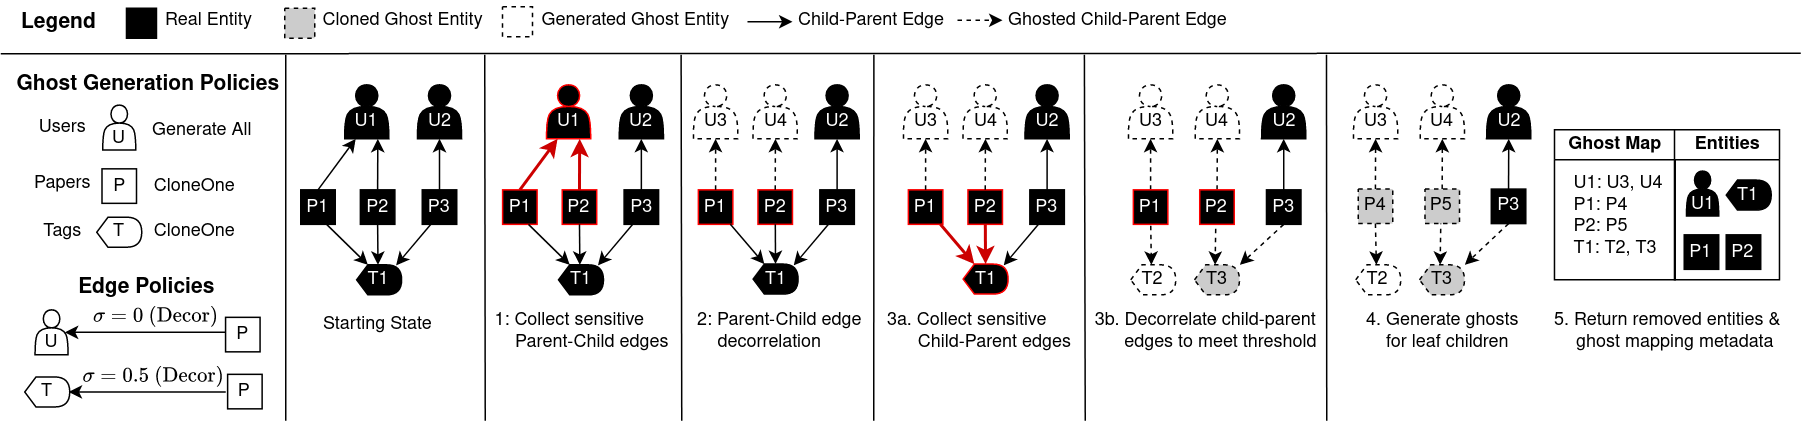
\includegraphics[width=.5\textwidth]{img/algo}
    \label{fig:algo}
    \caption{Examples of \sys's execution.}
\end{figure}

%\paragraph{Example policy.}
%We can imagine an application tin which only the sum of votes per story is ever queried by the application; clusters of
%votes around stories can therefore remain without leaking identifying information, and are thus
%assigned Policy 1, ``Do Not Decorrelate (Retain)''. 
%Decorrelation does propagate to the votes themselves, which are clustered by a \texttt{location} attribute; 
%this cluster by location can have a different decorrelation policy that generates ghost locations by
%randomizing the location, breaking up the cluster. 
%
